\documentclass{article}

\usepackage{fancyhdr}
\usepackage{extramarks}
\usepackage{amsmath}
\usepackage{amsthm}
\usepackage{amsfonts}
\usepackage{amssymb} % Equations
\usepackage{mathtools}
\usepackage{commath}
\usepackage{tikz}
\usepackage[plain]{algorithm}
\usepackage{algpseudocode}
\usepackage{adjustbox} % Used to constrain images to a maximum size 
\usepackage{xcolor} % Allow colors to be defined
\usepackage{enumerate} % Needed for markdown enumerations to work
\usepackage{geometry} % Used to adjust the document margins
\usepackage{textcomp} % defines textquotesingle
\usepackage[arrow,matrix,curve,cmtip,ps]{xy}
\usepackage{hyperref}

\usetikzlibrary{automata,positioning}

%
% Basic Document Settings
%

\topmargin=-0.45in
\evensidemargin=0in
\oddsidemargin=0in
\textwidth=6.5in
\textheight=9.0in
\headsep=0.25in

\linespread{1.1}

\pagestyle{fancy}
\lhead{\hmwkAuthorName}
\chead{\hmwkClass\ (\hmwkClassInstructor\ \hmwkClassTime): \hmwkTitle}
\rhead{\firstxmark}
\lfoot{\lastxmark}
\cfoot{\thepage}

\renewcommand\headrulewidth{0.4pt}
\renewcommand\footrulewidth{0.4pt}

\setlength\parindent{0pt}


%
% Create Problem Sections
%

\newcommand{\enterProblemHeader}[1]{
    \nobreak\extramarks{}{Problem \arabic{#1} continued on next page\ldots}\nobreak{}
    \nobreak\extramarks{Problem \arabic{#1} (continued)}{Problem \arabic{#1} continued on next page\ldots}\nobreak{}
}

\newcommand{\exitProblemHeader}[1]{
    \nobreak\extramarks{Problem \arabic{#1} (continued)}{Problem \arabic{#1} continued on next page\ldots}\nobreak{}
    \stepcounter{#1}
    \nobreak\extramarks{Problem \arabic{#1}}{}\nobreak{}
}

\setcounter{secnumdepth}{0}
\newcounter{partCounter}
\newcounter{homeworkProblemCounter}
\setcounter{homeworkProblemCounter}{1}
\nobreak\extramarks{Problem \arabic{homeworkProblemCounter}}{}\nobreak{}

%
% Homework Problem Environment
%
% This environment takes an optional argument. When given, it will adjust the
% problem counter. This is useful for when the problems given for your
% assignment aren't sequential. See the last 3 problems of this template for an
% example.
%
\newenvironment{homeworkProblem}[1][-1]{
    \ifnum#1>0
        \setcounter{homeworkProblemCounter}{#1}
    \fi
    \section{Problem \arabic{homeworkProblemCounter}}
    \setcounter{partCounter}{1}
    \enterProblemHeader{homeworkProblemCounter}
}{
    \exitProblemHeader{homeworkProblemCounter}
}

%
% Homework Details
%   - Title
%   - Due date
%   - Class
%   - Section/Time
%   - Instructor
%   - Author
%

\newcommand{\hmwkTitle}{Homework 03}
\newcommand{\hmwkDueDate}{Oct 11, 2018}
\newcommand{\hmwkClass}{Math 6366 Optimization}
\newcommand{\hmwkClassTime}{}
\newcommand{\hmwkClassInstructor}{Andreas Mang}
\newcommand{\hmwkAuthorName}{\textbf{Jonathan Schuba}}

%
% Title Page
%

\title{
    \textmd{\textbf{\hmwkClass:\ \hmwkTitle}}\\
    \normalsize\vspace{0.1in}\small{Due\ on\ \hmwkDueDate}\\
}
\author{\hmwkAuthorName}
\date{}

\renewcommand{\part}[1]{\textbf{\large Part \Alph{partCounter}}\stepcounter{partCounter}\\}

%
% Various Helper Commands
%

% Useful for algorithms
\newcommand{\alg}[1]{\textsc{\bfseries \footnotesize #1}}
% For derivatives
\newcommand{\deriv}[1]{\frac{\mathrm{d}}{\mathrm{d}x} (#1)}
% For partial derivatives
\newcommand{\pderiv}[2]{\frac{\partial}{\partial #1} (#2)}
% Integral dx
\newcommand{\dx}{\mathrm{d}x}
% Alias for the Solution section header
\newcommand{\solution}{\textbf{\large Solution}}


%-------------------------------------------
%       Begin Local Macros
%-------------------------------------------
\newcommand{\Gal}{\mathrm{Gal}}
\newcommand{\Aut}{\mathrm{Aut}}
\newcommand{\Prob}{\mathbf{P}}
\newcommand{\Pow}{\mathcal{P}}
\newcommand{\F}{\mathcal{F}}
\newcommand{\M}{\mathcal{M}}
\newcommand{\A}{\mathcal{A}}
\newcommand{\B}{\mathcal{B}}
\newcommand{\E}{\mathcal{E}}
\newcommand{\n}{\noindent}
\newcommand{\Z}{\mathbb{Z}}
\newcommand{\N}{\mathbb{N}}
\newcommand{\Q}{\mathbb{Q}}
\newcommand{\R}{\mathbb{R}}
\newcommand{\C}{\mathbb{C}}
\newcommand{\T}{\mathbb{T}}
\newcommand{\im}{\operatorname{im}}
\newcommand{\coker}{\operatorname{coker}}
\newcommand{\ind}{\operatorname{ind}}
\newcommand{\rank}{\operatorname{rank}}
\newcommand\mc[1]{\marginpar{\sloppy\protect\footnotesize #1}}
\newcommand{\ra}{\rangle}
\newcommand{\la}{\langle}
%-------------------------------------------
%       end local macros
%-------------------------------------------




\begin{document}

\maketitle

\begin{homeworkProblem}[1]
	Consider the optimization problem
	\[
	\begin{aligned}
		\underset{x\in\R^2}{\text{minimize}} \quad & f_0(x) \\ 
		\text{subject to} \quad & 2x_1+x_2\ge 1 \\ 
		& x_1+3x_2\ge 1 \\ 
		& x_1 \ge 0 \\ 
		& x_2 \ge 0
	\end{aligned} 
	\]
	Make a sketch of the feasible set. 
	
	\begin{figure}[h]
		\centering
		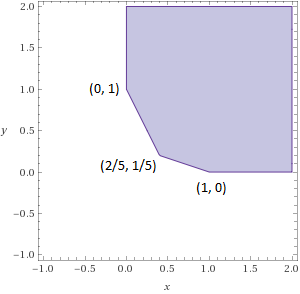
\includegraphics[width=0.4\linewidth]{image/q01}

	\end{figure}

		
	For each of the following objective functions, give the optimal set and
	the optimal value.
	\begin{enumerate}[a)]
		\item $f_0(x) = x_1 + x_2$.
		\subitem {The optimal point is $(2/5, 1/5)$ and the optimal value is $3/5$. By inspection.}
		
		\item $f_0(x) = \max \{x_1,x_2\}$.
		\subitem { The optimal point is $(1/3, 1/3)$ and the optimal value is $1/3$. By inspection.}
		
		\item $f_0(x) = x_1^2 + 9x_2^2$.
		\subitem {The optimal point is $(1/2, 1/6)$ and the optimal value is $1/2$. Using the CVX program. (This is the 21st century, after all.)}
		
	\end{enumerate}

	
\end{homeworkProblem}

\begin{homeworkProblem}[2]
	Verify that $x^* = \begin{bmatrix}1 \\	0.5 \\ 	-1	\end{bmatrix} $ is optimal for the optimization problem
	\[
	\begin{aligned}
	\underset{x\in\R^3}{\text{minimize}} \quad & \frac{1}{2}x^\top A x +q^\top x + r \\
	\text{subject to} \quad & -1 \le x_i \le 1, i = 1,2,3
	\end{aligned}
	\]

	where $A = \begin{bmatrix}
	13& 12& -2 \\ 12& 17& 6 \\ -2& 6& 12	
	\end{bmatrix}$ , $q = \begin{bmatrix}
	-22 \\ -14.5 \\ 30
	\end{bmatrix}$ and $r = 1$.
	
	\textbf{Solution:}
	
	This is a quadratic, convex objective, so the optimal value occurs when the gradient is zero.
	
	\[ \nabla f_0(x) = Ax + q^\top = 0 \]
	\[
	\nabla f_0(x^*) = \begin{bmatrix}
	13& 12& -2 \\ 12& 17& 6 \\ -2& 6& 12	
	\end{bmatrix} * x^* + \begin{bmatrix}
	-22 \\ -14.5 \\ 30
	\end{bmatrix}^\top = \begin{bmatrix}-1 \\	0 \\ 	19	\end{bmatrix}
	\]
	So, at $x^*$, the gradient is not zero in all directions.  But the objective value only gets better for increasing $x_1$ and decreasing $x_3$, which would put us outside of the constraints.  The gradient for $x_2$ is zero, so the value of $x_2$ is optimal here. 
	
	
\end{homeworkProblem}

\begin{homeworkProblem}[3]
	content...
\end{homeworkProblem}

\begin{homeworkProblem}[4]
	Consider the unconstrained optimization problem
	\[
	\begin{aligned}
	\underset{x\in\R^n}{\text{minimize}} \quad & \|A(x)\|_2 \\
	\end{aligned}
	\]

	where $\|A\|_2$ is the spectral norm and $A(x) = A_0 + \sum_{i=1}^{n}A_i$. Derive the equivalent semidefinite program. Use the fact that $A^\top A \succeq s^2 I$, where $I = \text{diag}(1,\dots, 1) \in \R^{n,n}$.
		
	\textbf{Solution:}
	
	This is an example on Page 169-170 of the textbook.  In the textbook, they say that $\|A\|_2 \le s$ if and only if  $A^\top A \preceq s^2 I$, so I'm going to use it like that. I'm just copying the textbook solution here.
	
	Then, we can express the problem as:
	\[
	\begin{aligned}
	\underset{s, x}{\text{minimize}} \quad & s \\
	\text{subject to} \quad & A(x)^\top A(x) \preceq sI
	\end{aligned}
	\]
	We bring in the fact that:
	\[
	A^\top A \preceq t^2I \ (\text{and}\ t \ge 0) \leftrightarrow \begin{bmatrix}
	tI & A \\ A^\top &tI 
	\end{bmatrix} \succeq 0
	\]
	And we get the semi-definite program
		\[
	\begin{aligned}
	\underset{t, x}{\text{minimize}} \quad & t \\
	\text{subject to} \quad &  \begin{bmatrix}
	tI & A \\ A^\top &tI 
	\end{bmatrix} \succeq 0
	\end{aligned}
	\]
	
\end{homeworkProblem}

\begin{homeworkProblem}[5]
	Consider the vector optimization problem with respect to the positive semidefinite cone
	\[
	\begin{aligned}
	\underset{X \in S^n_+}{\text{minimize}} \quad & X \\
	\text{subject to} \quad & X \succeq A_i, \quad i=1,\dots,m
	\end{aligned}
	\]
	where $A_i \in S^n, i = 1,\dots, m$, are given. State the minimization problem if you were to apply scalarization
	to solve this problem.
	
	\textbf{Solution:}
	
	This is an example on page 180 of the textbook.  Please assume that I could easily copy it here.
\end{homeworkProblem}

\begin{homeworkProblem}[6]
	Let $A \in \R^{m,n}$, $x \in \R^n$, and $b \in \R^m$. Formulate the following problems as linear programs. Explain in	detail the relation between the optimal solution of each problem and the solution of its equivalent linear program.
	
	\begin{enumerate}[a)]
		\item minimize $\|Ax-b\|_\infty$ (unconstrained $\ell^\infty$-norm approximation).
			\subitem {
				The infinity-norm is the absolute value of the largest element in the vector.  So, we can introduce a new variable, $r$, whose absolute value cannot be lower than that of the largest element in $Ax-b$.  We minimize over $r$ and $x$.
				\[
				\begin{aligned}
				\underset{r\in\R, x\in\R^n}{\text{minimize}} \quad & r \\
				\text{subject to} \quad & -r \le a_i^\top x - b_i \le r,\quad i = 1,2,\dots,m
				\end{aligned}
				\]
				
				This is equivalent to $t \ge \max_{i} |a_i^\top x - b_i|$.
			}
		
		
		\item minimize $\|Ax-b\|_1$ (unconstrained $\ell^1$-norm approximation).
			\subitem{
			The one-norm is the sum of the absolute values of the elements, so we introduce a vector $r$, whose elements are no less than the absolute values of the elements of $Ax-b$.  We minimize the sum of elements in $r$.
			\[
			\begin{aligned}
			\underset{r\in\R^m, x\in\R^n}{\text{minimize}} \quad & \sum_{i=1}^m r_i \\
			\text{subject to} \quad & -r_i \le a_i^\top x - b_i \le r_i,\quad i = 1,2,\dots,m
			\end{aligned}
			\]
			}
		
		\item minimize $\|Ax-b\|_1$ subject to $\|x\|_\infty \le 1$.
			\subitem This is the same as the previous solution, with one additional constraint: 
				\[
				\begin{aligned}
			\underset{r\in\R^m, x\in\R^n}{\text{minimize}} \quad & \sum_{i=1}^m r_i \\
				\text{subject to} \quad & -r_i \le a_i^\top x - b_i \le r_i, &i = 1,2,\dots,m\\
										& -1 \le x_j \le 1 & j = 1,2,\dots,n
				\end{aligned}
				\]
	\end{enumerate}


\end{homeworkProblem}

\begin{homeworkProblem}[7]
	Let the induced/operator norm of the $\ell^\infty$ vector norm, denoted by $\|\cdot\|_\infty : \R^{m,n} \to \R$, be given by
	\[
	\|A\|_\infty = \sup_{x\ne 0} \frac{	\|Ax\|_\infty}{	\|x\|_\infty}	= \max_{i=1,\dots,m} \sum_{j=1}^{n}|a_{ij}|
	\]
	This norm is sometimes called the max-row-sum norm. Consider the problem of approximating a matrix,
	in the max-row-sum norm, by a linear combination of other matrices. That is, we are given $k + 1$ matrices
	$A_i \in \R^{m,n}, i = 0,\dots, k$, and need to find $x \in \R^k$ that minimizes
	\[
	\|A_0 + \sum_{i=1}^{k}x_i A_i\|_\infty
	\]
	Express this problem as a linear program. Explain the significance of any extra variables in your linear
	program. Carefully explain how your program formulation solves this problem, e.g., what is the relation
	between the feasible set for your linear program and this problem?
	
	\textbf{Solution:}
	
	Let $A(x) = A_0 + \sum_{i=1}^{k}x_i A_i$, and let $a_{ij}$ be the entries of $A(x)$.  This problem is can be first expressed as a non-convex problem: 
	\[
	\begin{aligned}
	\underset{x\in\R^k}{\text{minimize}} \quad & \max_{i=1,\dots,m} \sum_{j=1}^{n}|a_{ij}| &\\
	\end{aligned}
	\]
	
	Let us introduce a new variable, $t \in \R$, and reformulate the problem:
	\[
	\begin{aligned}
	\underset{t\in\R, x\in\R^k}{\text{minimize}} \quad & t &\\
	\text{subject to} \quad &  \sum_{j=1}^{n}|a_{ij}| \le t & \text{for}\ i = 1,\dots,m
	\end{aligned}
	\]
	Here, the optimal choice for $t$ is equivalent to the infinity norm, for a given $x$. The optimization program will find the optimal $x$ for which $t$ is lowest. We can now get rid of the absolute value by introducing a matrix, $S$, which is constrained by $A(x)$.
	\[
	\begin{aligned}
	\underset{t\in\R, x\in\R^k}{\text{minimize}} \quad & t &\\
	\text{subject to} \quad &  \sum_{j=1}^{n}s_{ij} \le t & \text{for}\ i = 1,\dots,m\\
							&  -S \preceq A(x) \preceq S
	\end{aligned}
	\]  
	The curly inequalities are element-wise between the matrices $S$ and $A(x)$.
	
	
	
	
\end{homeworkProblem}

\pagebreak


\begin{homeworkProblem}[8]
	We consider a linear dynamical system with state $x(t) \in \R^n, t = 0,\dots, n_t$, and actuator or input signal
	$u(t) \in \R$ for $t = 0,\dots, n_t − 1$. The dynamics of the system are given by the linear recurrence
	\[
	x(t + 1) = Ax(t) + bu(t),\quad t = 0,\dots, nt − 1,
	\]
	where $A \in \R{n,n}$ and $b \in \R^n$ are given. We assume that the initial state is zero, i.e., $x(0) = 0$. The
	minimum fuel optimal control problem is to choose the inputs $u(0), ..., u(nt − 1)$ so as to minimize the
	total fuel consumed, which is given by $f = \sum_{t=0}^{n_t-1} f (u(t))$ subject to the constraint that $x(n_t) = x_{des}$,	where $n_t$ is the (given) time horizon, and $x_{des}\in \R^n$ is the (given) desired final or target state. The function $f : \R \to \R$ is the fuel use map for the actuator, and gives the amount of fuel used as a function of the actuator signal amplitude. In this problem we use
	\[
	f(a) = \begin{cases} 
			|a| & |a| \le 1 \\
			2|a|-a & |a| > 1 
			\end{cases}
	\]

	This means that fuel use is proportional to the absolute value of the actuator signal, for actuator signals
	between -1 and 1; for larger actuator signals the marginal fuel efficiency is half. Formulate the minimum
	fuel optimal control problem as an linear program.
	
	\textbf{Solution:}
	
	Consider the location at each time step
	\[
	\begin{aligned}
	x_0 &= 0\\
	x_1 &= b u_0\\
	x_2 &= Ax_1+bu_1 = Abu_0 + bu_1\\
	x_3 &= A^2bu_0 + Abu_1 + bu_2\\
	\dots\\
	x_n &= A^{n-1} bu_0 + A^{n-2}bu_1 + \dots + Abu_{n-1} +  bu_n\\
	\end{aligned}
	\]
	Let us construct a matrix $M$, as follows:
	\[
	M = \begin{bmatrix}
		A^{n-1} b & A^{n-2}b & \dots & Ab & b
	\end{bmatrix}
	\]
	So that:
	\[
	x_n = Mu
	\]
	We will introduce an optimization variable, $t \in \R^n$, and formulate the problem as follows:
	\[
	\begin{aligned}
	\underset{t\in\R^n, u\in\R^n}{\text{minimize}} \quad & \sum_{i=1}^n t_i &\\
	\text{subject to} \quad &  Mu = x_{des}\\
							&  -t \preceq u \preceq t \\
							& -\frac{t+1}{2} \preceq u \preceq \frac{t+1}{2}
	\end{aligned}
	\]  
	The last two component-wise inequalities encode the fuel consumption function. 
	
\end{homeworkProblem}

\pagebreak

\begin{homeworkProblem}[9]
	Consider the quadratically constrained quadratic program
	\[
	\begin{aligned}
	\underset{}{\text{minimize}} \quad & 1/2 x^\top A x + q^\top x + r &\\
	\text{subject to} \quad &  x^\top x \le 1\\
	\end{aligned}
	\]  
	with $A\in S^n_{++}$. Show that $x^* = −(A + \lambda I)^{-1} q$ where $\lambda = max\{0, \hat{\lambda}\}$ $\hat{\lambda}$ is the largest solution of the nonlinear equation $q^\top (A + \lambda I)^{-2}q = 1$.
	
	\textbf{Solution:}
	
	The gradient is $Ax+q$.  Setting the gradient to zero, we have $x^* = A^{-1}(-q)$.  This solution only holds if $\|x^*\|_2 < 1$. That is, $x$ is strictly inside the constraint.  
	
	Otherwise, we have $\|x^*\|_2 = 1$, and the constraint prevails. In that case, $x$ satisfies $(P+\lambda I)x=-q$ for some $\lambda > 0$.  We must have that $x^*$ also satisfies $\|x^*\|_2 = \|(P+\lambda I)^{-1}q\|_2 = 1$.  Simplifying, we have:
	\[
	\begin{aligned}
	1 	&= \|(P+\lambda I)^{-1}q\|_2 \\
		&= ((P+\lambda I)^{-1}q)^\top (P+\lambda I)^{-1}q\\
		&= q^\top (P+\lambda I)^{-2}q
	\end{aligned}
	\]
	
	So, either $\lambda=0$, and $x$ is strictly inside the constraints, or $x^\top x = 1$ and $\lambda$ must satisfy the aforementioned equation. 
\end{homeworkProblem}

\begin{homeworkProblem}[10]
	Express the geometric program
	\[
	\begin{aligned}
	\underset{x}{\text{minimize}} \quad & \max \{ p(x), q(x) \} &\\
	\end{aligned}
	\] 
	where p and q are posynomials, as a convex optimization problem.
	
	\textbf{Solution:}
	\[
	\begin{aligned}
	\underset{x,\ t}{\text{minimize}} \quad & t &\\
	\text{subject to} \quad &  p(x) \le t\\
							&  q(x) \le t
	\end{aligned}
	\] 
	And one can then use the appropriate logarithm change of variables for the posynomials.
	
	
\end{homeworkProblem}


\end{document}
